\documentclass[12pt]{article}
\usepackage[utf8]{inputenc}
\usepackage[french]{babel}
\usepackage{pdfpages, tabto, amsmath, graphicx, xcolor}
\usepackage[margin = 1in]{geometry}
\usepackage[colorlinks=true, allcolors=blue]{hyperref}

\begin{document}

\begin{titlepage}
    \begin{center}
    
\includegraphics[width= 17 cm]{ensimag.png} 
    \end{center}
    \begin{center}
        \vspace{2cm}
        \large Projet Génie Logiciel
        \vspace{0,5\baselineskip}
        {\Large\textbf{Charte d'équipe}\\
        \vspace*{1\baselineskip}
        \Large\textbf{Fait par les étudiants}}
        \vspace{1\baselineskip}\\
        Mohamed Hadi \bsc{Chamsi} \\Li \bsc{Rong}\\Oussama \bsc{Lamzaouri}\\Ziad \bsc{Razani}\\ Safia \bsc{Echarif} \\
		\vspace{3.5\baselineskip}
		Janvier 2022
    \end{center}
\end{titlepage}

\newpage

\begin{abstract}
Composée de cinq membres, notre équipe se veut complète et très motivée pour le projet GL.
Une variété des origines de formation :
Trois étudiants ayant fait leur première année à l’ENSIMAG.
Deux autres de Phelma Grenoble-inp en filière SEOC.\\
\end{abstract}


\section{\textbf{Compétences et points forts des membres de l’équipe :}}
Pour résumer les compétences de l’équipe, on propose la matrice SWOT suivante :

 \begin{figure}[h]
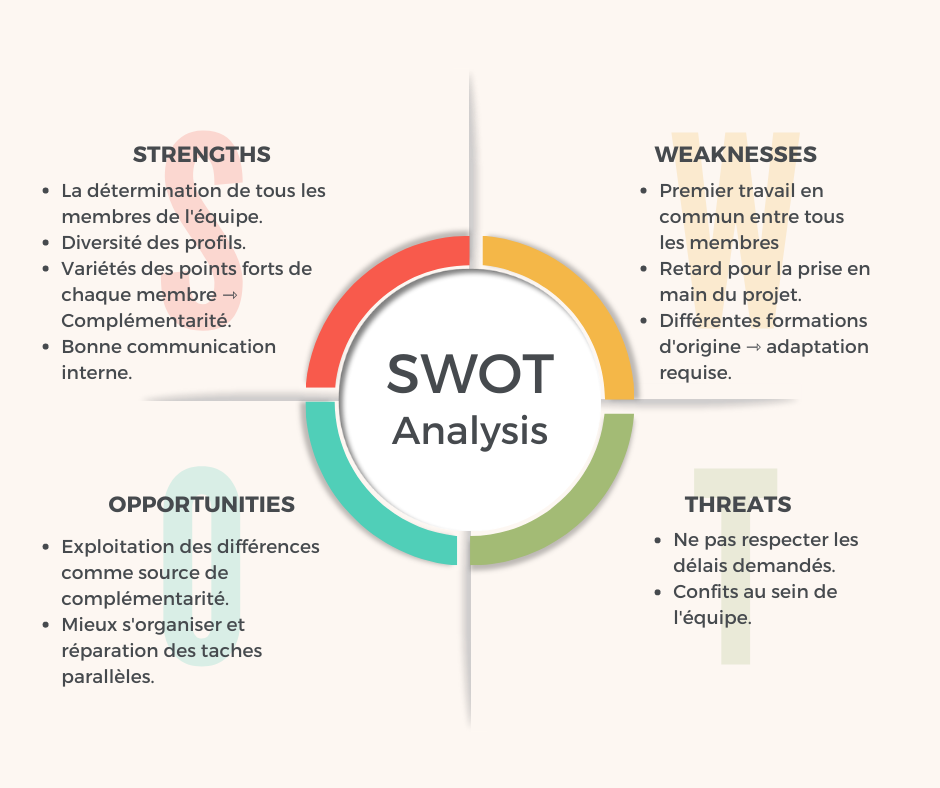
\includegraphics[width=1.1\textwidth]{swot.png}
\centering
\end{figure}

\newpage

\section{\textbf{Valeurs Communes :}}

Pour la réussite d’un travail en groupe et une bonne cohésion équipe, il est nécessaire de partager quelques valeurs communes entre les membres afin de faciliter la communication interne. 
En l'occurrence, notre équipe est fondée sur le respect des membres et le partage des idées ainsi qu’une communication saine et efficace pour l’avancement du projet. 
Non seulement cela, mais on définit un règlement intérieur pour éviter tout conflit au sein de notre équipe. On cite: \ \begin{itemize}
    \item Ponctualité vis-à-vis des réunions.
    \item Droit à l’erreur.
    \item Être digne des tâches confiées et en assumer la responsabilité.
    \item Partage de toutes les ressources et informations via notre groupe Discord.
\end{itemize}


\section{\textbf{Rôles et responsabilités dans l’équipe:}}
La répartition des rôles et responsabilités a été fait en se basant sur les fiches d'autoevaluation fourni par les membres d'équipe. Néanmoins, il ne sont pas définitifs (rôles tournants) et pourront être changer, si besoin, durant le déroulement du projet.
\subsection{les Rôles :}
On définit les rôles ont été réparties entre les membres ( voir \ref{tab1}) comme suit :
\begin{itemize}
    \item Chef de projet : suit l'avancement du projet, et supervise les différentes phases du projet.
    \item Secrétaire : anime les réunions et rédige les comptes rendus de celles-ci.
    \item Pôle Communication : chargé de la communication interne et externe. Vérifie que la communication se passe au sein de l'équipe, se charge également de la communication avec le tuteur et de la communication écrite.
    \item Pôle Qualité : Assure la qualité des codes, tests et tout autre document. 
    \item Pôle Développement : Conçoit, développe et met en application les scripts et les programmes décrites sur le cahier des charges.
\end{itemize}
\begin{center}
\resizebox{18cm}{!}{
    \begin{tabular}{|c|c|}
     \hline
    Rôles & Membres  \\ \hline
    Chef de projet & Oussama \bsc{Lamzaouri}\\ \hline
    Secrétaire & Safia \bsc{Echarif}\\ \hline
    Pôle Communication &  Oussama \bsc{Lamzaouri}, Mohamed Hadi \bsc{Chamsi}, Ziad \bsc{Razani} \\ \hline
    Pôle Qualité (tests) & Ziad \bsc{Razani},  Li \bsc{Rong}   \\ \hline
    Pôle Développement & Oussama \bsc{Lamzaouri}, Ziad \bsc{Razani}, Mohamed Hadi \bsc{Chamsi}, Safia \bsc{Echarif}, Li \bsc{Rong}  \\ \hline
    \end{tabular} 
        \label{tab1}
}
\end{center}

\subsection{Responsabilités}
Comme il y a pas mal de tâches à réaliser, il nous est apparu judicieux de désigner un responsable pour chaque incrément (ou étape) et pour la validation. 
La répartition des responsabilités est schématisé par le tableau suivant: 
\begin{center}
\resizebox{11cm}{!}{
    \begin{tabular}{|c|c|}
     \hline
    Membres & Responsabilités  \\ \hline
    Li \bsc{Rong} & Responsable Etape A \\ \hline
    Oussama \bsc{Lamzaouri} & Responsable Etape B\\ \hline
    Mohamed Hadi \bsc{Chamsi} & Responsable Etape C \\ \hline
    Safia \bsc{Echarif} & Responsable Validation\\ \hline
    Ziad \bsc{Razani} &  Responsable Git \\ \hline
    \end{tabular} 
}
\end{center}

\section{\textbf{Communication au sein de l’équipe :}}
\subsection{organiation et outils de communication }
Généralement, nous travaillons en groupe à l'ensimag,
 mais comme il y a une grande partie de travail qu'on fait chez nous, et étant donné la situation sanitaire courante, il nous a paru pertinet d'envisager d'autres outils de communication à distance : Discord en plus d'une conversation sur messenger, en plus d'échanger nos contacts (adresses mails et numéros de téléphone). \\
 En ce qui concerne la gestion des documents, nous avons le git déjà fourni par les encadrants, mais, comme ce n'est pas très pratiques pour des fichiers txt, et tex, nous avons pensé à créer un drive où on met tout les fichiers utiles comme cette charte en plus des documentations et google docs crées, et de créer des fichiers dans overleaf permettant l'écriture synchrone des fichiers .tex (y compris les documentations). 
\subsection{Les règles de communication :}
Pour éviter tout conflit entre les membres de l'équipe, on a instauré un ensemble de règles qui doivent étre impérativement respecter par chaque membre de l'équipe :
\begin{itemize}
    \item chaque membre doit se tenir au courant de l'évolution du projet.
    \item chaque membre doit communiquer toute information potentiellement utile au groupe.
    \item En cas de conflit, les membres concernés doivent aller voir le chef de projet pour en parler calmement, si le conflit concerne toute l'équipe, la secrétaire devra fixer une réunion pour l'aborder toujours dans le cadre du respect d'autrui.
\end{itemize}
\subsection{Les réunions :}

Nous consacrerons régulièrement $30$ à $45$  min par jour  (généralement avant de quitter l'ensimag) pour une réunion afin de mettre le point sur l'avancement du projet et pour mettre à jour notre planning. la secrétaire est chargée de les animer er de rédiger un compte rendu qui sera mis sur le drive. \\

\section{\textbf{Fiches d'autoevaluation des membres de l’équipe :}}
Vous trouverez ci-dessus les fiches d’autoevaluation des membres de l’equipe.
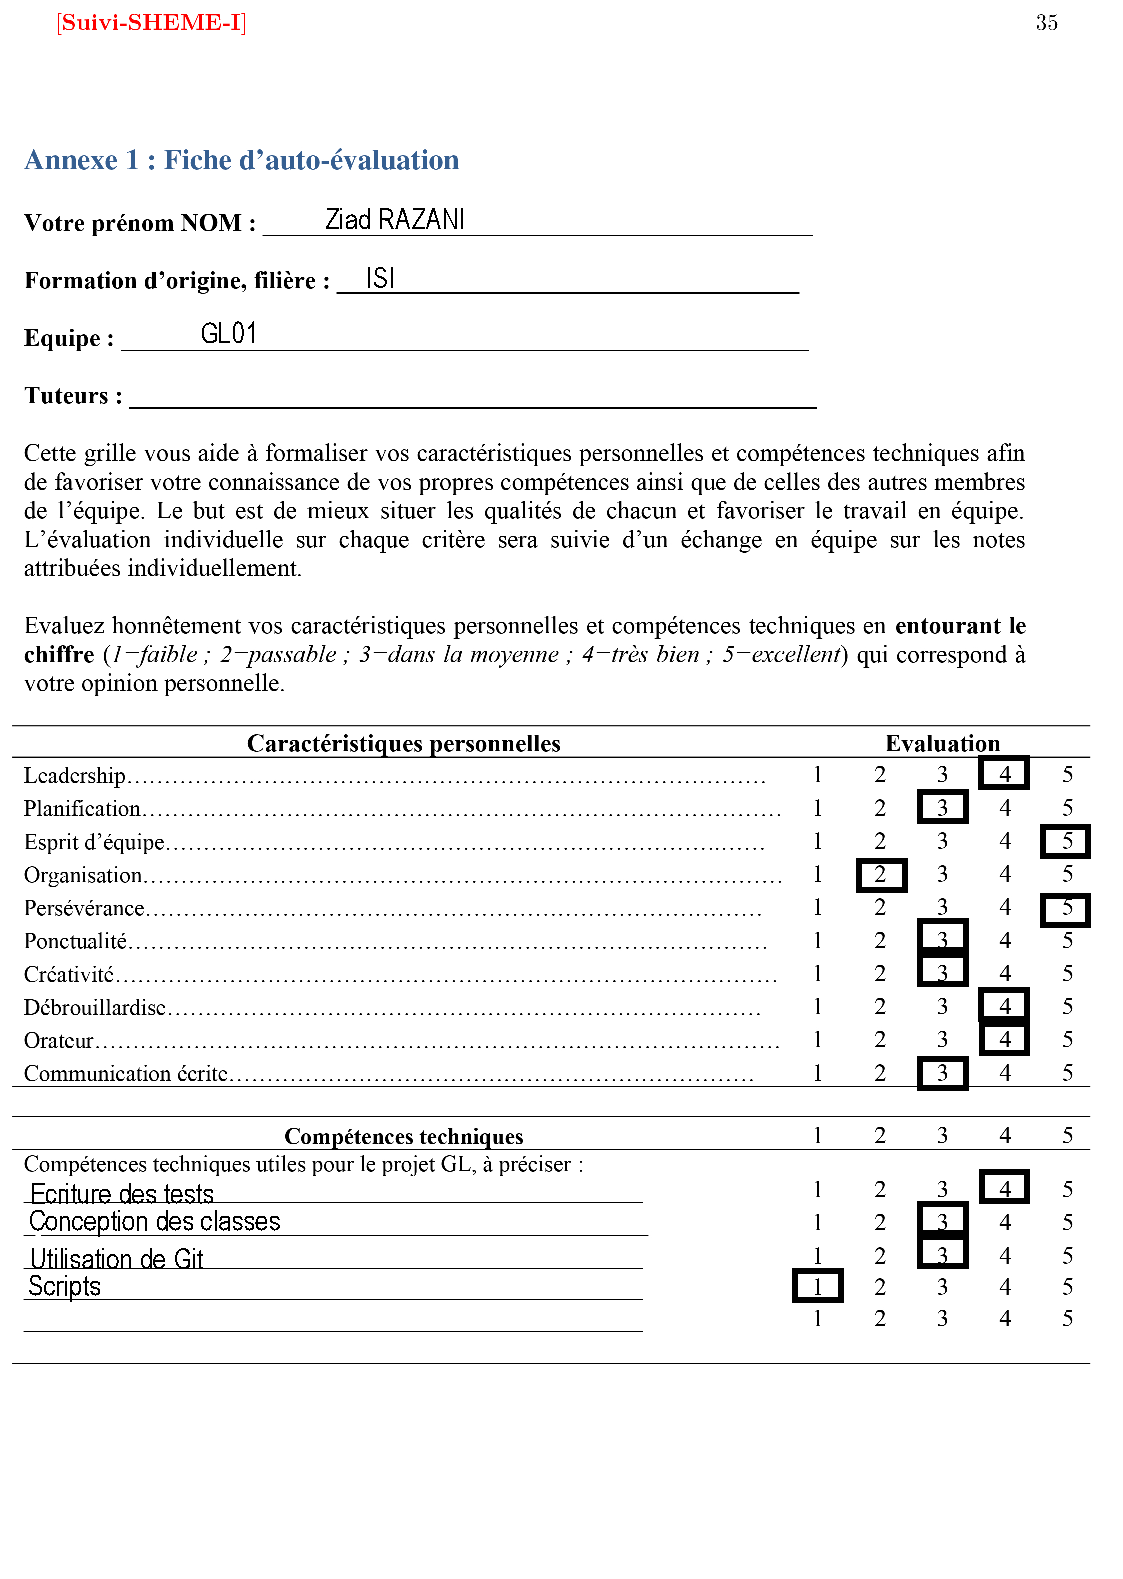
\includepdf[pages=-]{fiche-ziad-razani.pdf}
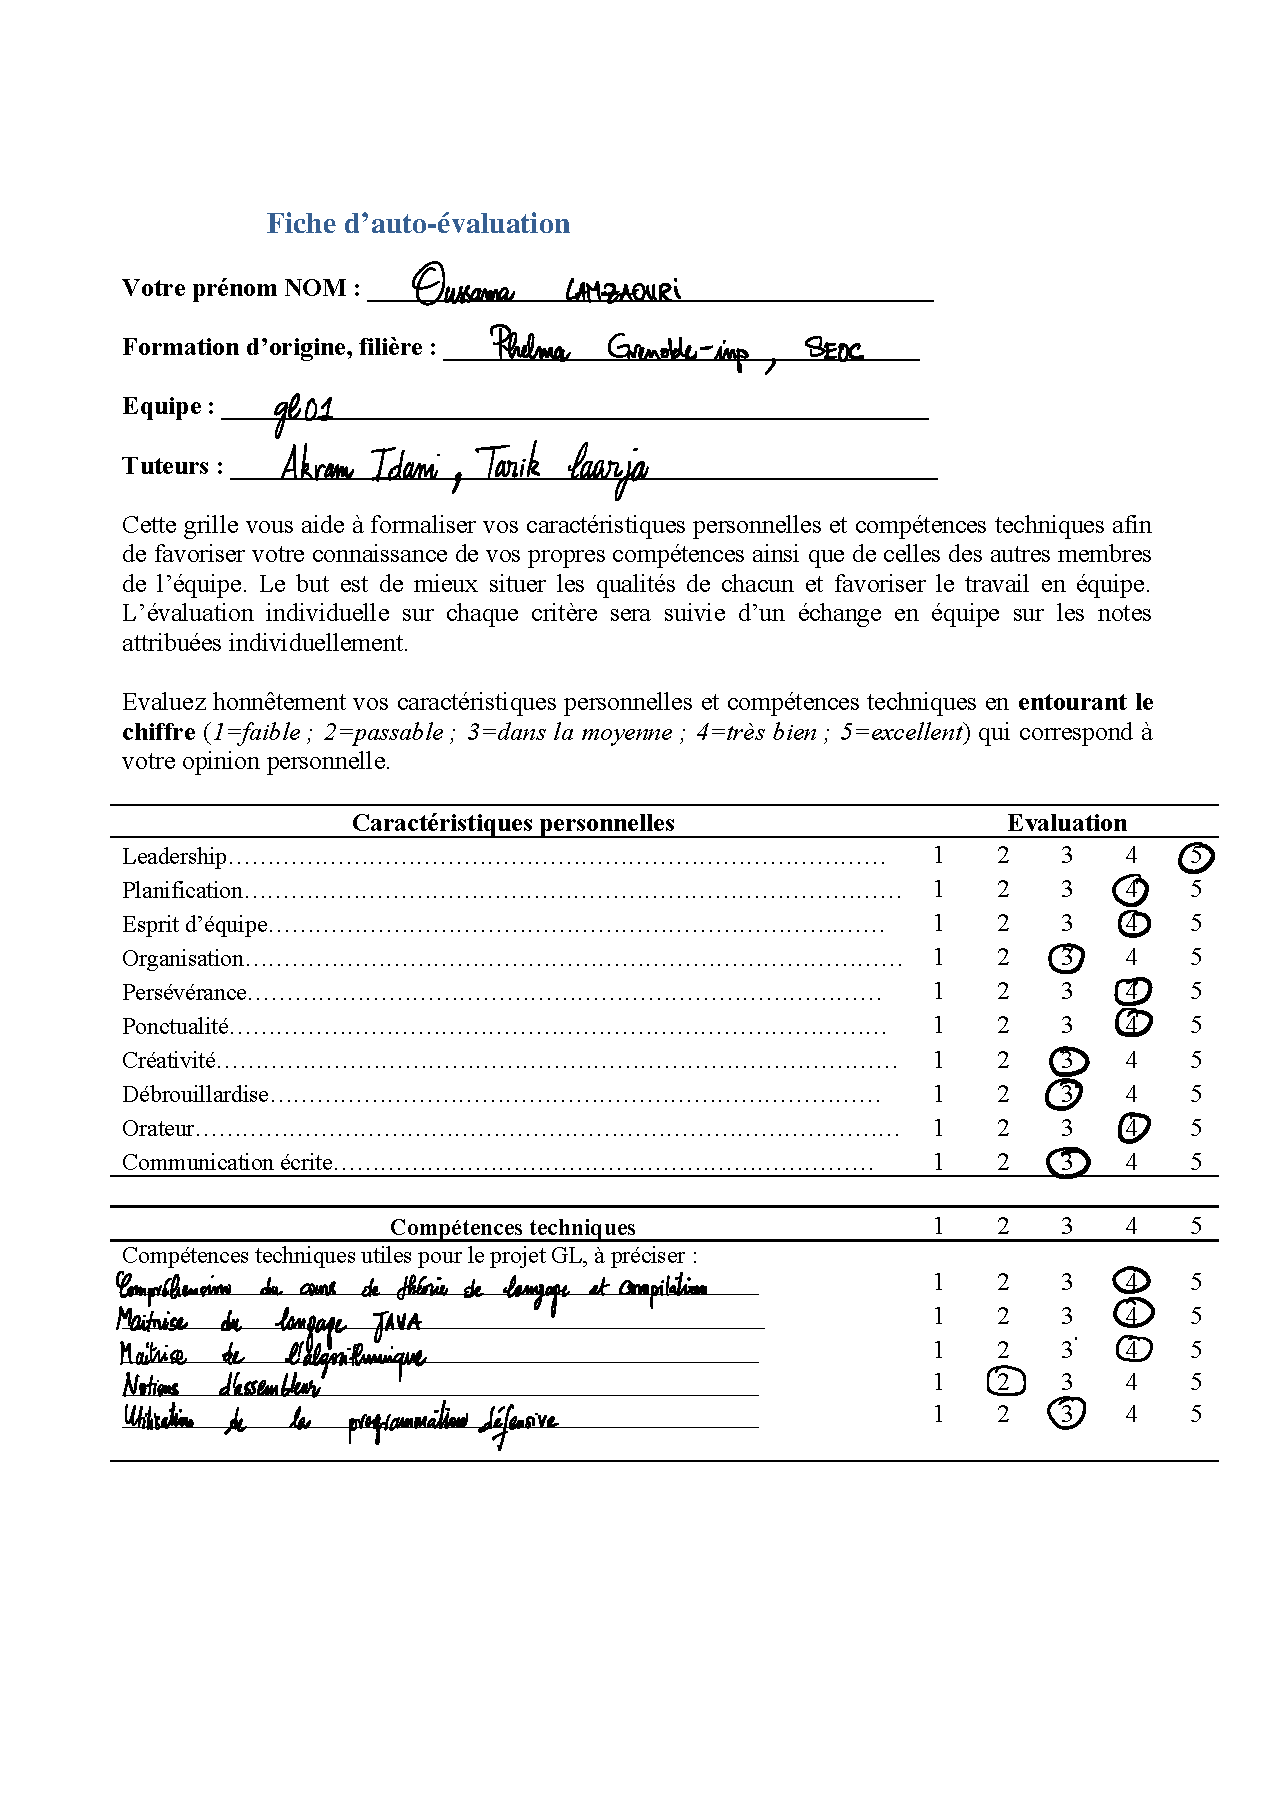
\includepdf[pages=-]{fiche_oussama.pdf}
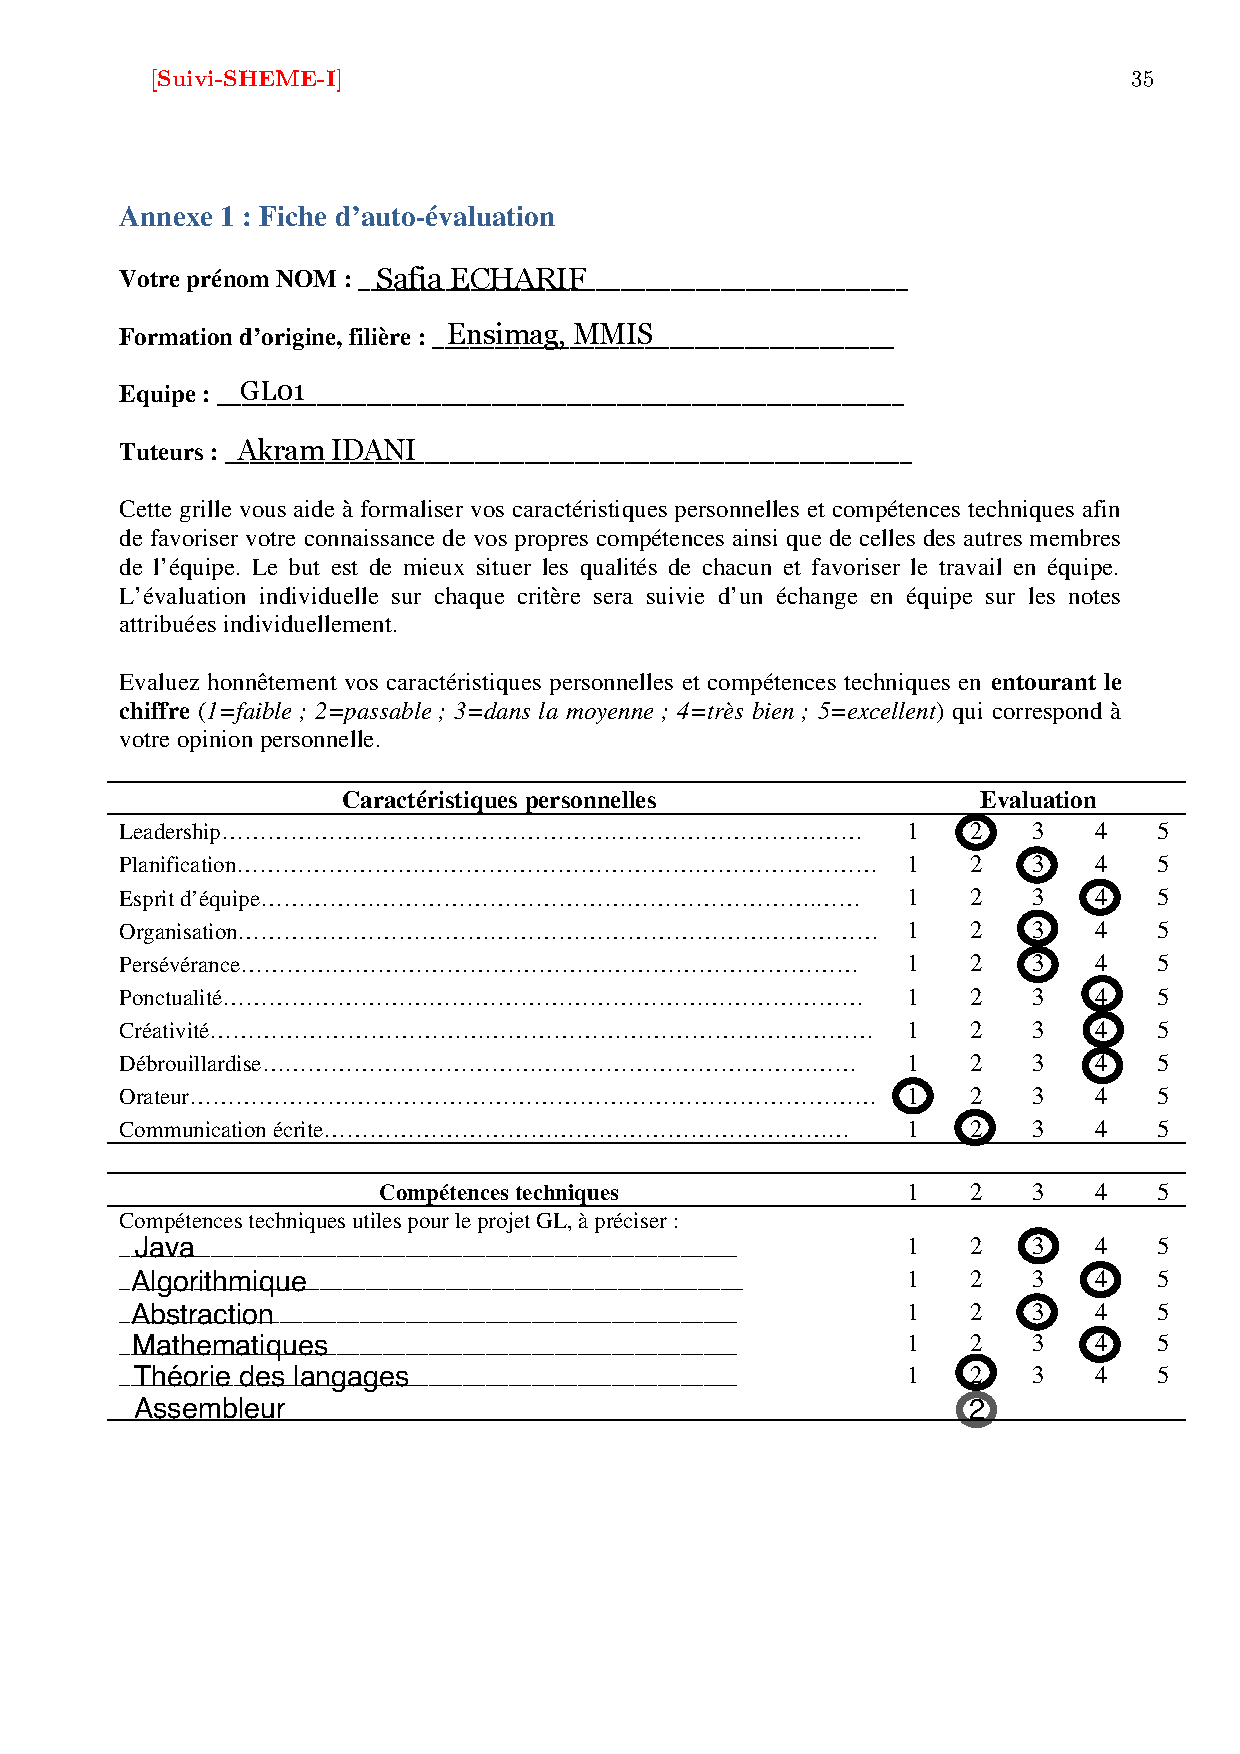
\includepdf[pages=-]{fiche_safia.pdf}
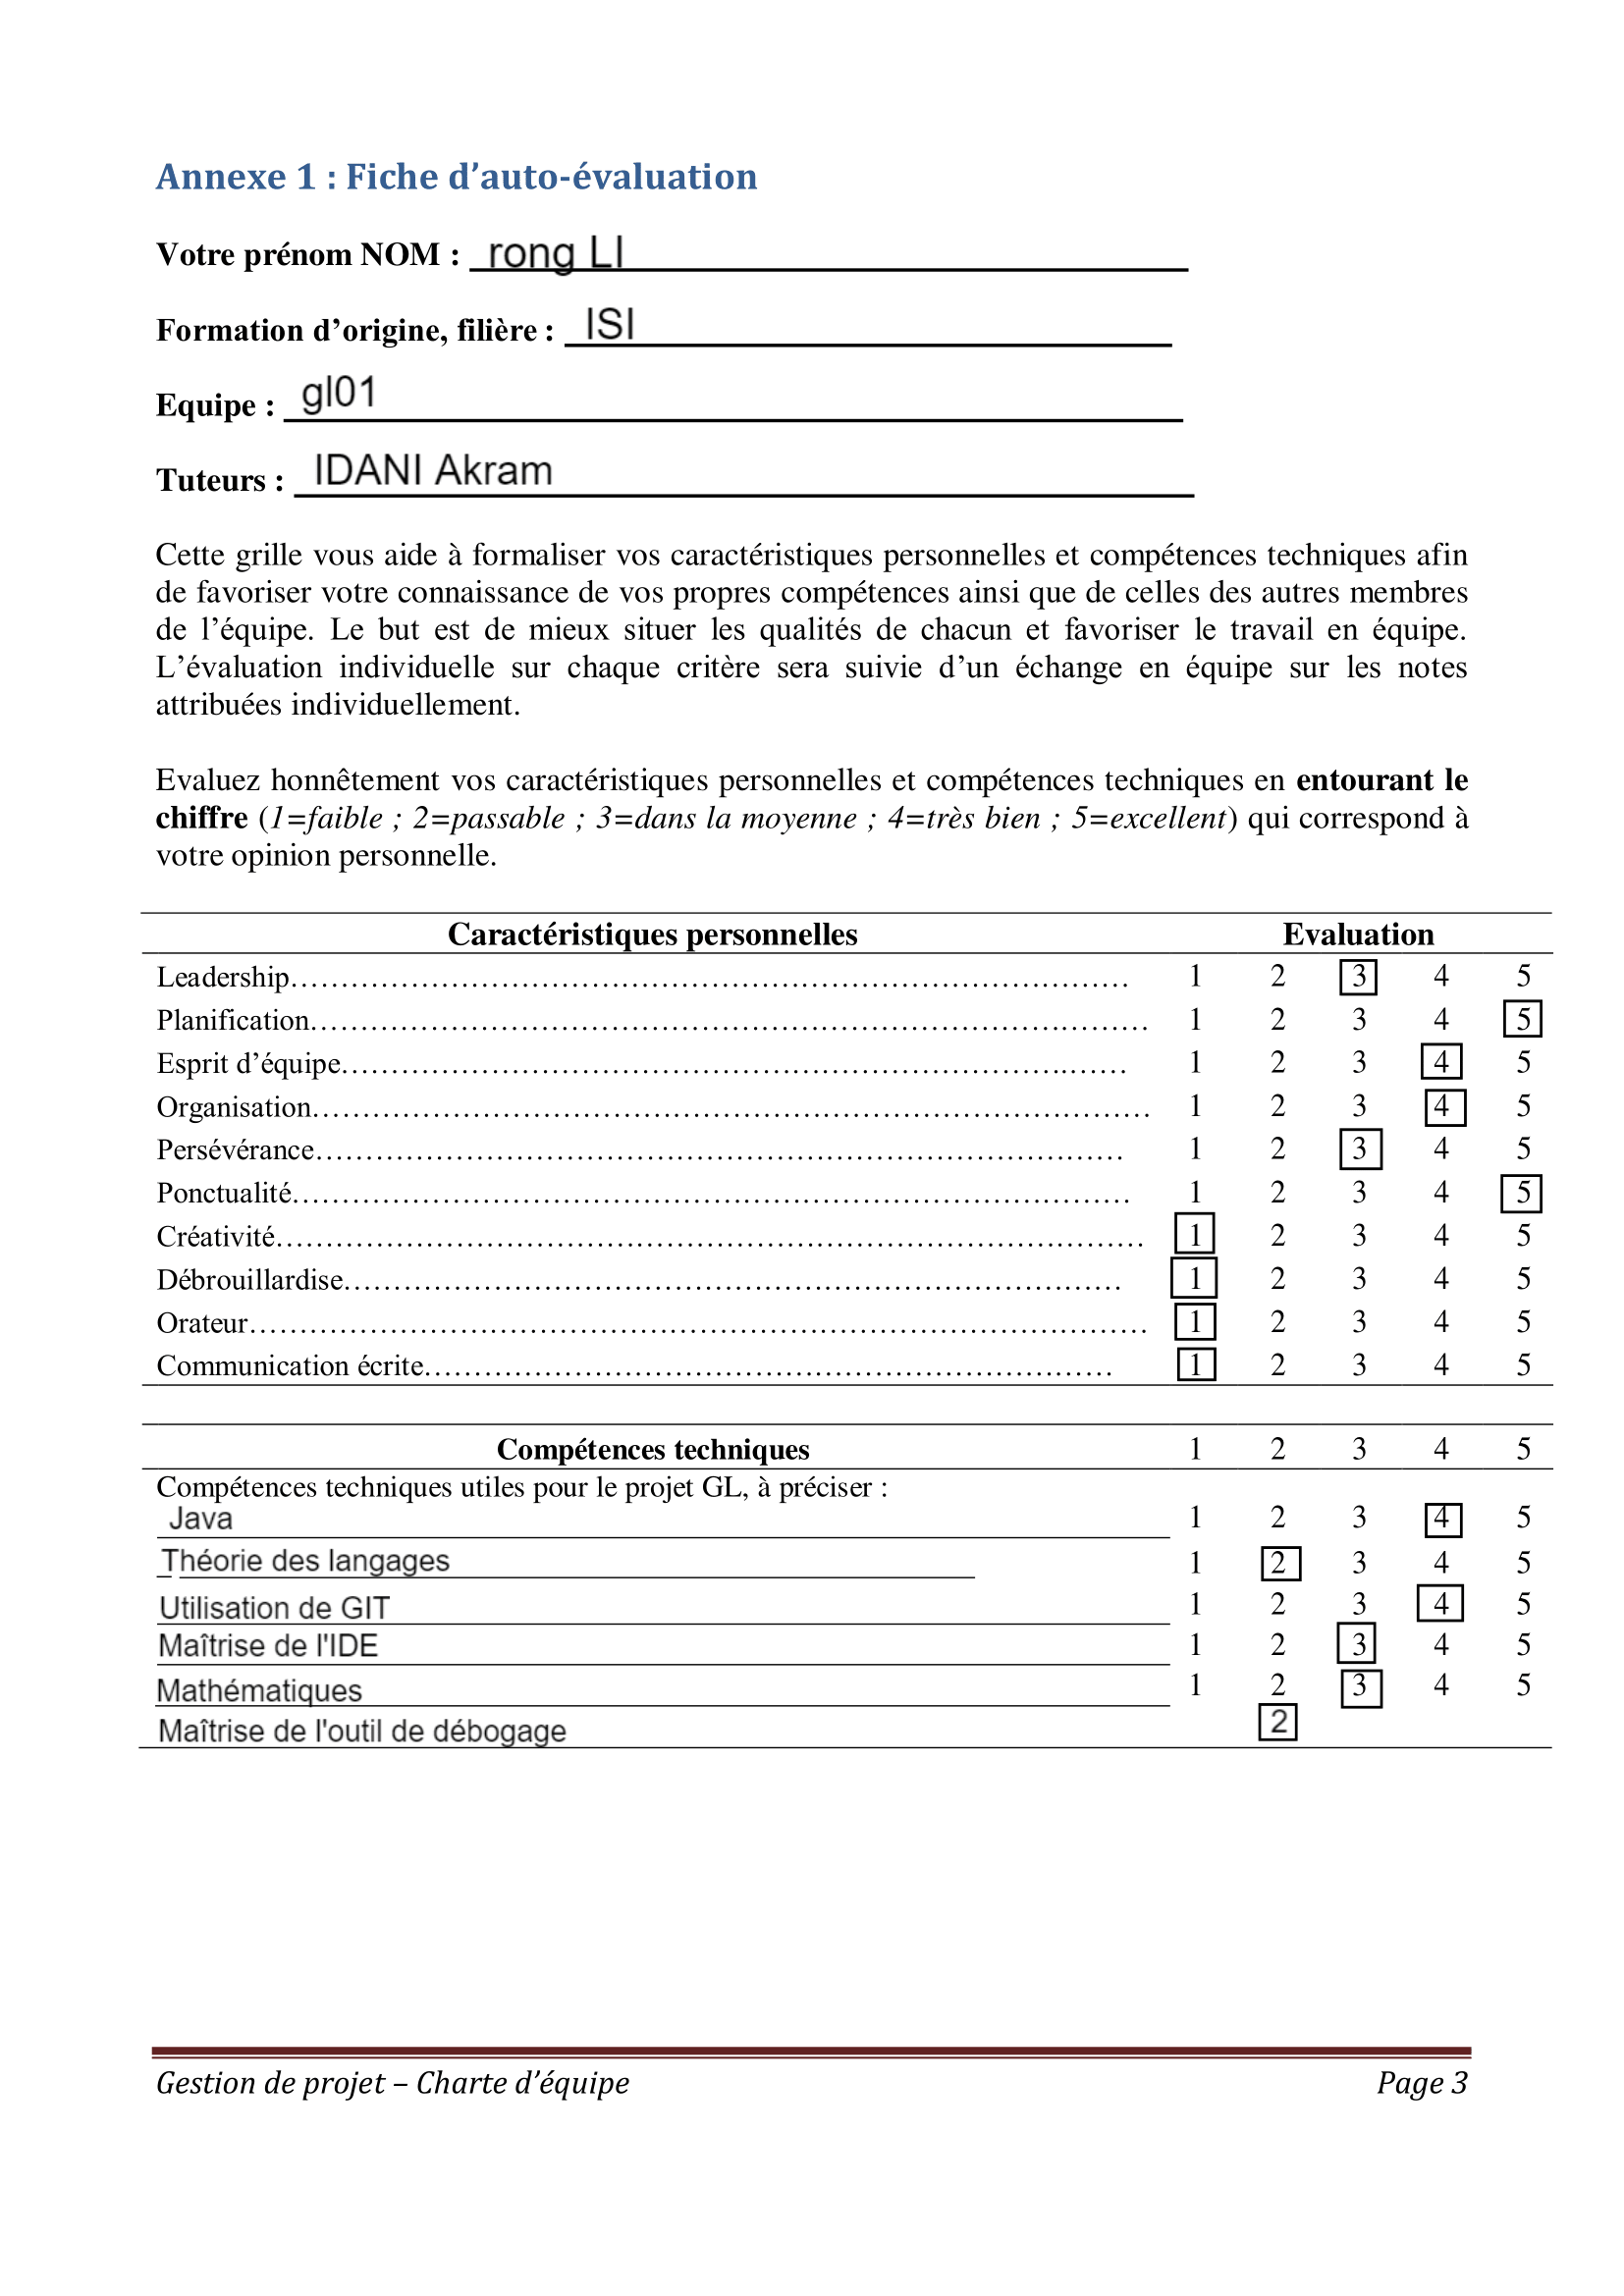
\includepdf[pages=-]{fiche-auto-Rong-1.png}
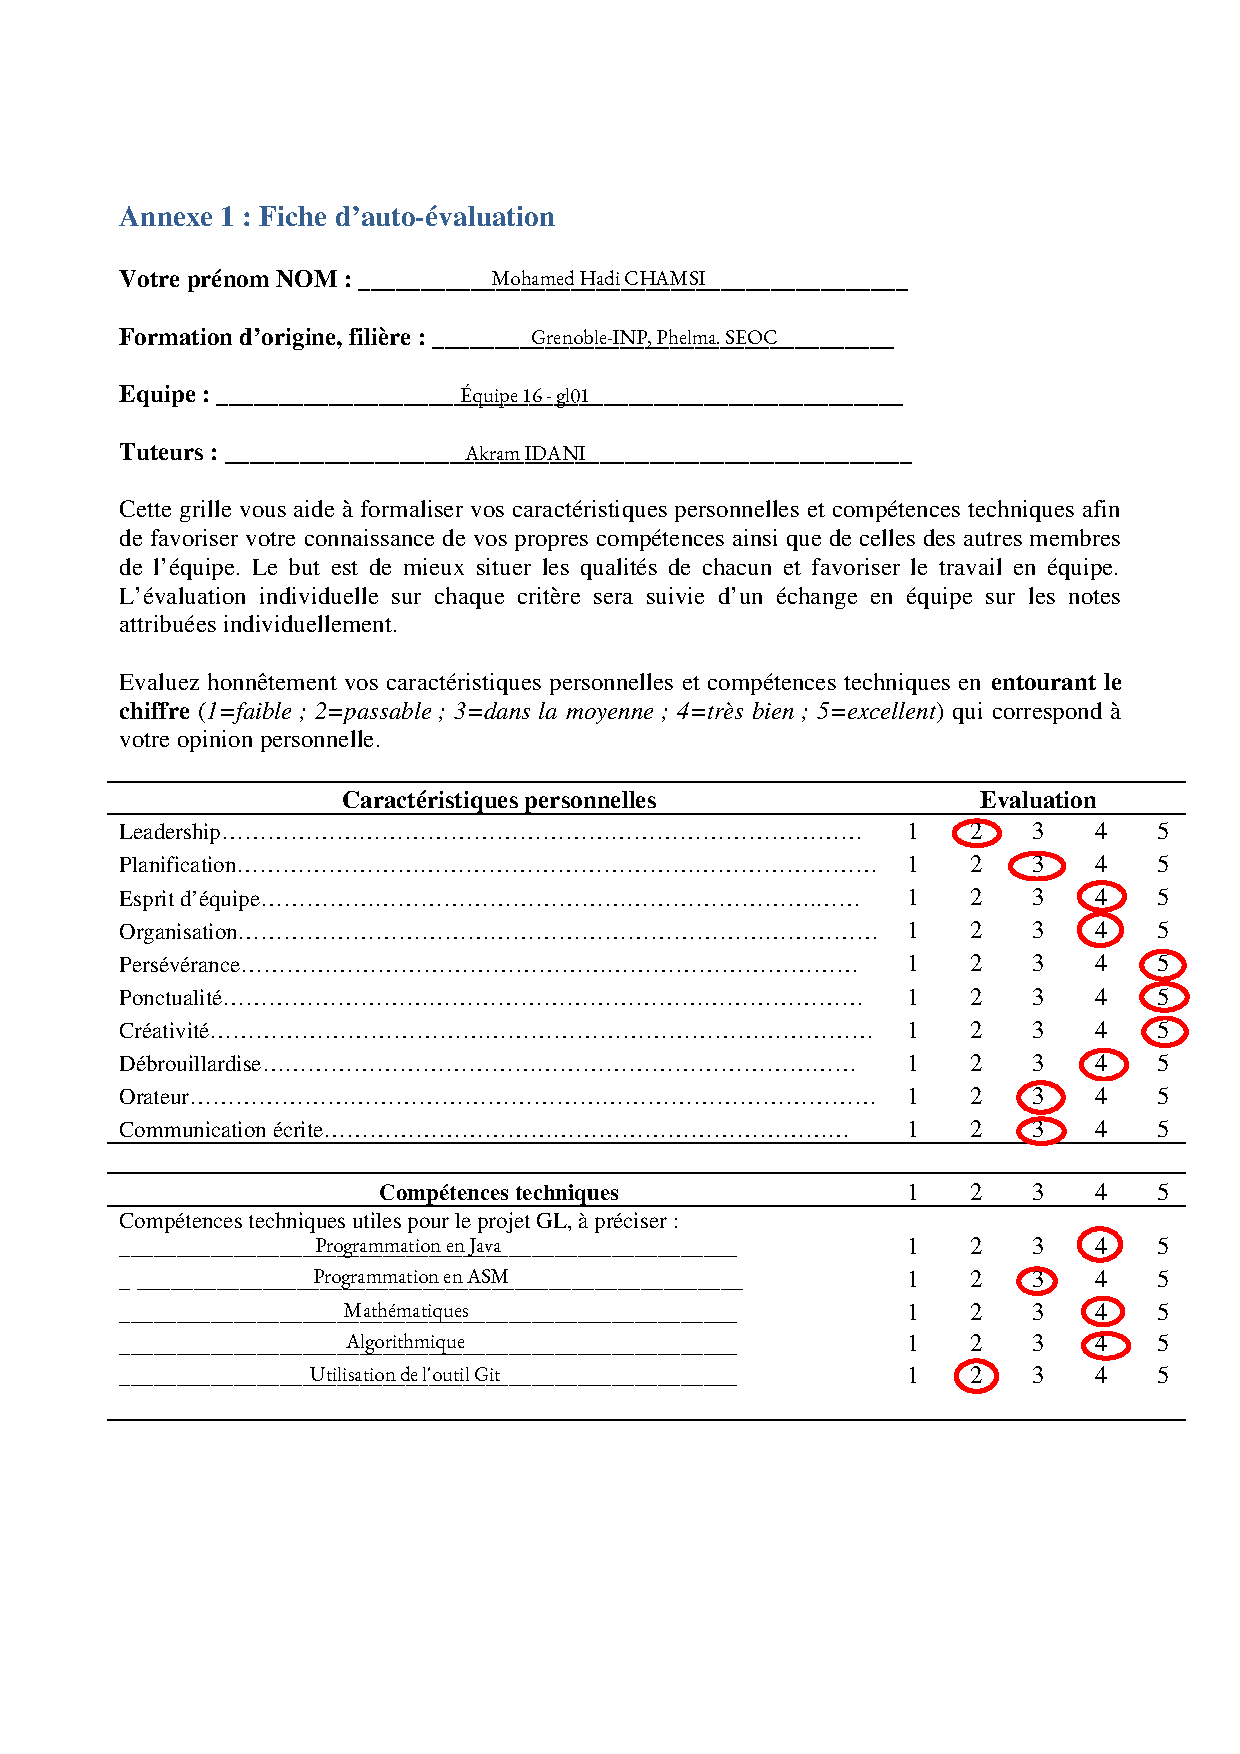
\includepdf{fiche_chamsim.pdf}


\end{document}
